\section{Realizzazione}
    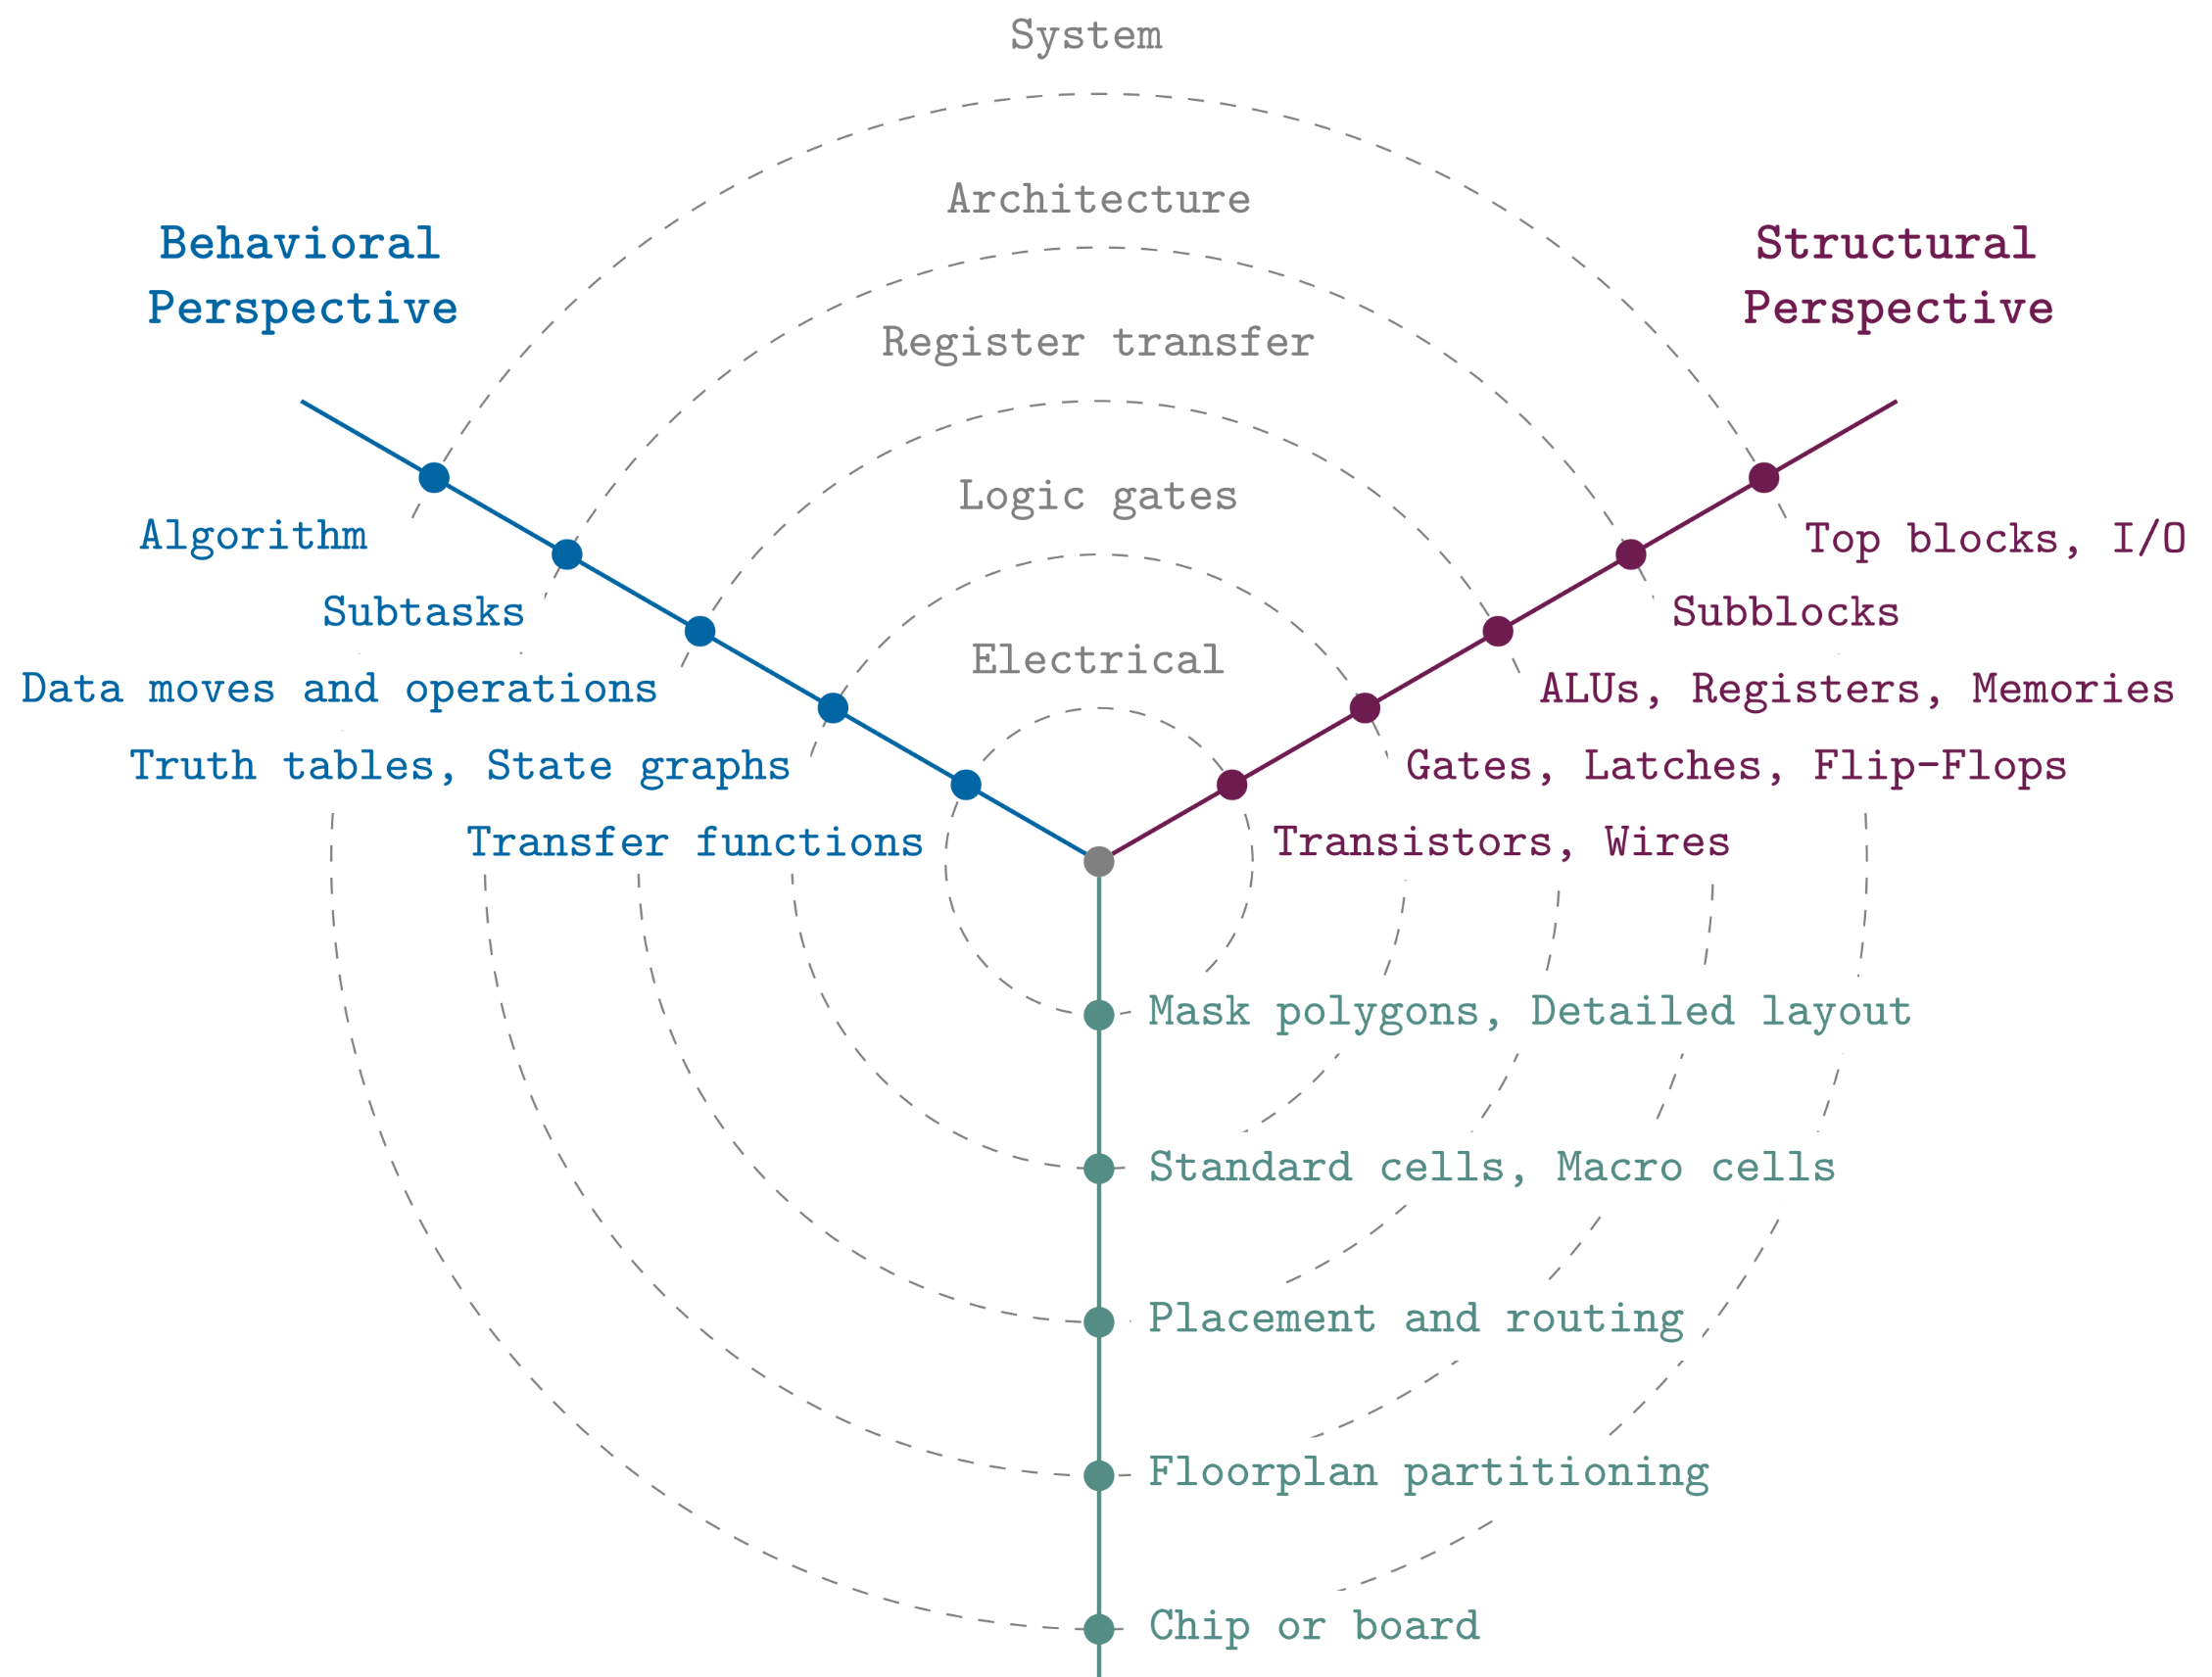
\includegraphics[width=0.5\columnwidth]{Images/Development model.png}
    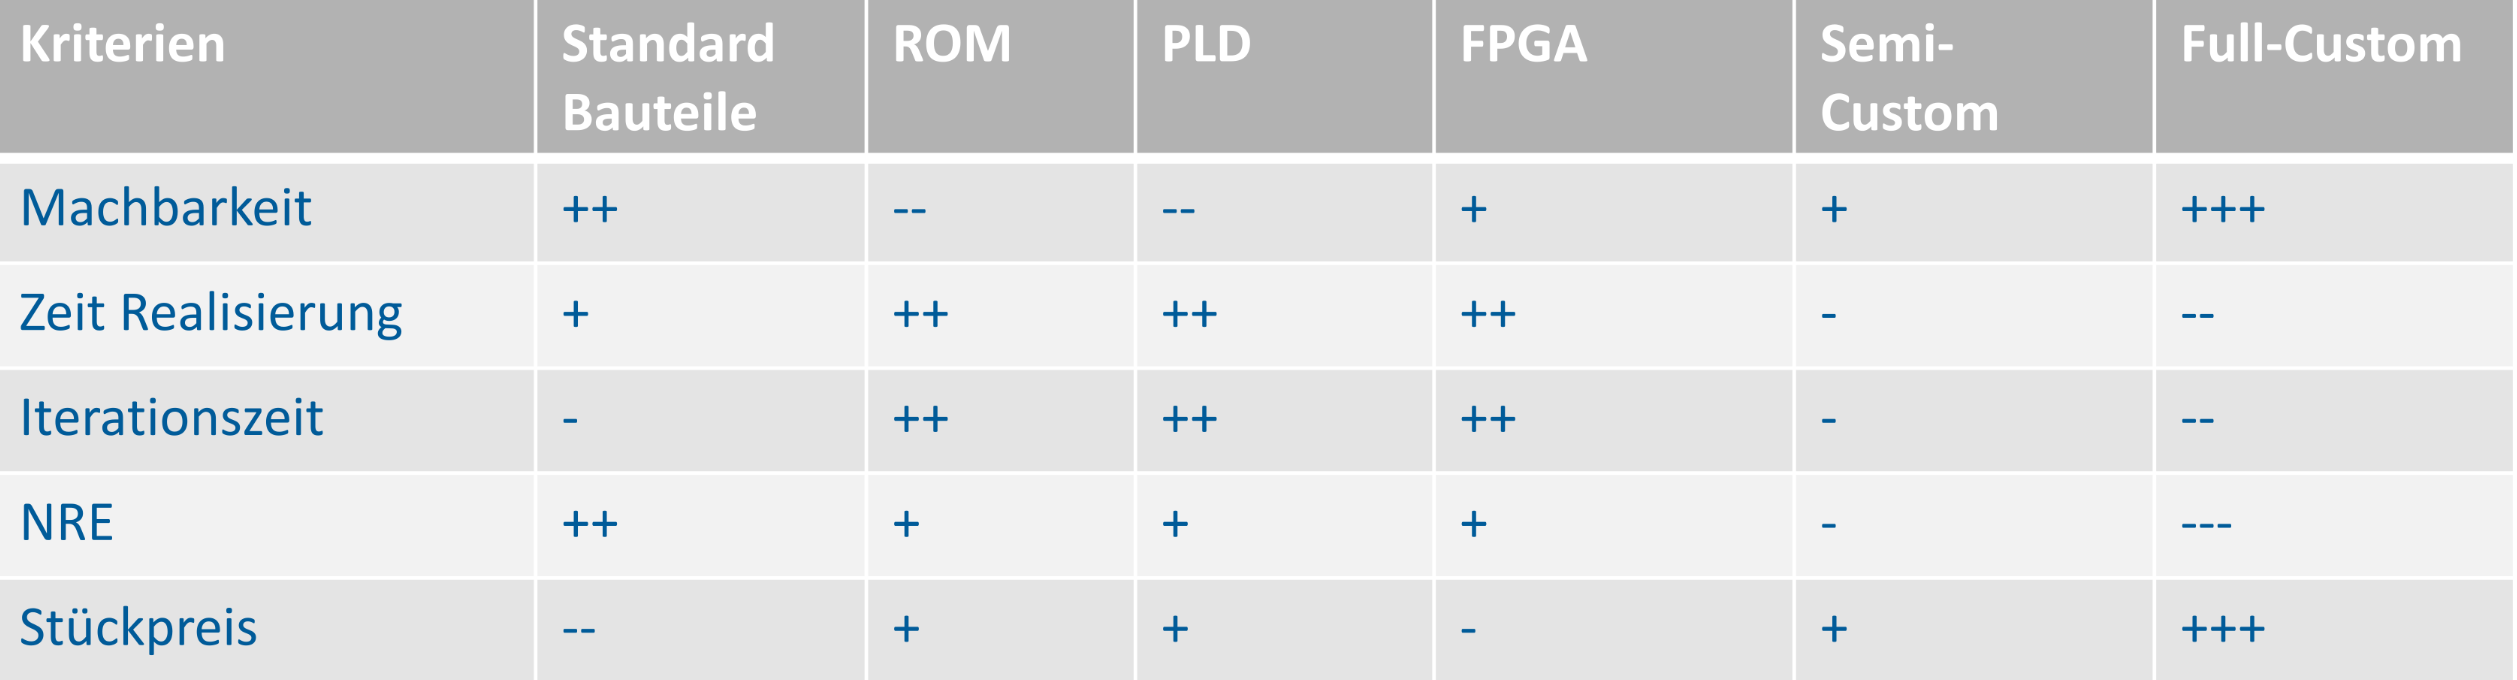
\includegraphics[width=0.5\columnwidth]{Images/Whal der realisirungsform.png}

\section{Processi}
    I processi sono sezioni di codice che vengono eseguite ogni volta che un \textcolor{red}{Segnale} nella lista sensibile cambia.
    % Inizia un codice blocco, con colori VHDL (vedi definizione in DigDes.tex), escape inside is used to use external commands
    \begin{lstlisting}[language=VHDL, escapeinside={(*@}{@*)}]
    process (clk, reset, (*@\textcolor{red}{SegnaliSensibili}@*)) 
        begin
            if reset = '1' then
                -- codice di reset
            elsif rising_edge(clk) then
                -- codice di clock
            end if;
        end process;
    \end{lstlisting}